% !TeX program = xelatex

\documentclass{BFSU-master-thesis}

% ---------------------------基本信息----------------------------------

\UJSsetup{
title       = {Write the long English title right here please},
titlerownum = 2,   % 首页封面标题的行数
runtitle    = {中文题目},
author      = {你的名字},
major       = {学科名称},
advisor     = {指导老师},
jobtitle    = {教授},
ReplyDate   = {2024年06月},
chairman    = {学院名称},
date        = {2024年6月6日},
}

\begin{document}

% ---------------------------封面声明----------------------------------

\frontmatter

\maketitle             % 生成封面

\makeauthorization     % 独创性和授权书

% ---------------------------中文摘要----------------------------------

\begin{cnabstract}
这是使用\LaTeX{}编写的北京外国语大学硕士毕业论文模板,由江苏大学硕士学位论文模板修改而来。
(非官方的,官方没有模板) 修改者为 Ryan-the-hito,原作者为 Tex 白兔。

摘要字数不要超过三页。

\zhlipsum[1-2]     % 中文乱假文

\cnkeywords{铁进称,规例本百型支,色战红元,话质应,保反易,投今联,适光自气,布见么务,西准感,办省林罐}
\end{cnabstract}

% ---------------------------英文摘要----------------------------------

\begin{enabstract}

This is a dissertation template of Jiangsu University written in \LaTeX{}.

The number of words in the abstract should not exceed three pages.

\lipsum[1-3]

\enkeywords{Pellentesque; Habitant morbi; Tristique senectus; Et netus et; Malesuada fames; Ac turpis egestas; Donec odio elit}

\end{enabstract}

% ---------------------------目录插图----------------------------------

\tableofcontents      % 目录生成

\listoffigures        % 生成插图目录

\mainmatter

% ---------------------------正文开始----------------------------------

\chapter*{绪\quad 论}
\addcontentsline{toc}{chapter}{绪\quad 论}

\zhlipsum[1-1]

\subsection{一级标题}

\zhlipsum[1-1]

\subsubsection{二级标题}

\zhlipsum[1-2]

\paragraph{三级标题}

\zhlipsum[1-1]

\chapter{简介}

\begin{quote}
“\LaTeX{}是应该是世界上目前最专业的论文写作软件,有很完备的系统,以及数千的宏包支持,许多顶级期刊只接收\TeX{}格式的投稿,很多大学都有官方的\LaTeX{}模板。在中国\LaTeX{}的使用并不算普遍,为了方便之后课程论文的写作,同时推广\LaTeX{}的使用,编写了此模板。”
\end{quote}


文档测试平台 TeXLive2021  + Win10,修改后测试平台 Texifier + macOS 12.6.8

编译方式 xelatex

\section{重要声明}

\begin{itemize}
\item 任何个人和团体可以无限制的自由使用和更改此模板
\item 本模板为非官方模板,模板作者对使用该模板所引起的后果不负任何责任
\end{itemize}

有问题联系邮箱 sweeter.02.implant@icloud.com

\section{基本使用方式}

正如他文中所写,“既不隐瞒,也不宣告,而是仅仅指点”。\footnote{尼采著,李秋零译:《不合时宜的沉思》,华东师范大学出版社,2007 年 1 月版,第 238 页。}

伯林追问:“但是为更高的地位而斗争、希望摆脱低下的地位,应该被称作为自由而斗争吗?把这个词限定在上面讨论过的那些意义内仅仅是学究气吗?要么,我怀疑,我们是不是要冒这种危险,把人类所赞赏的他的社会境况的任何改善都称作他的自由的增长,从而使这个词变得太含糊、太宽泛,以致使它实质上没有用处?另一方面,我们又不能简单地将这种情况斥为纯粹的概念混淆一将自由观念与地位、团结、友爱、平等观念或这些观念的某种联合混淆。因为,对地位的渴望,在某些方面,非常类似于成为独立的行动者的欲望。”\footnote{以赛亚·伯林著,胡传胜译:《自由论》,译林出版社,2011 年 3 月版,第 208 页。}

\subsection{一级标题}

\zhlipsum[1-1]

\subsubsection{二级标题}

\zhlipsum[1-3]     % 中文乱假文

\chapter{一些环境的使用}

\section{公式使用}
\ding{172} 一行公式~\eqref{eq1}
\begin{align}
\label{eq1}
a^2+b^2=c^2
\end{align}
其中xxx

\ding{173} 二行公式~\eqref{eq2}
\begin{align}
\label{eq2}
a^2+b^2=c^2\\
\label{eq3}
a^2+b^2=c^2
\end{align}
其中xxx

\ding{174} 分段公式~\eqref{eq4}
\begin{align}
\label{eq4}
|x| =
\begin{cases}
-x & \text{if } x < 0,\\
0 & \text{if } x = 0,\\
x & \text{if } x > 0.
\end{cases}
\end{align}
其中xxx

\section{图使用}

双语标题使用 \verb|\bicaption{}{}|命令;图~\ref{fig2-1}

\begin{figure}[h!t]
\centering
\subfigure[子图标题一]{
\includegraphics[width=0.45\linewidth]{example-image-a}}\quad
\subfigure[子图标题二]{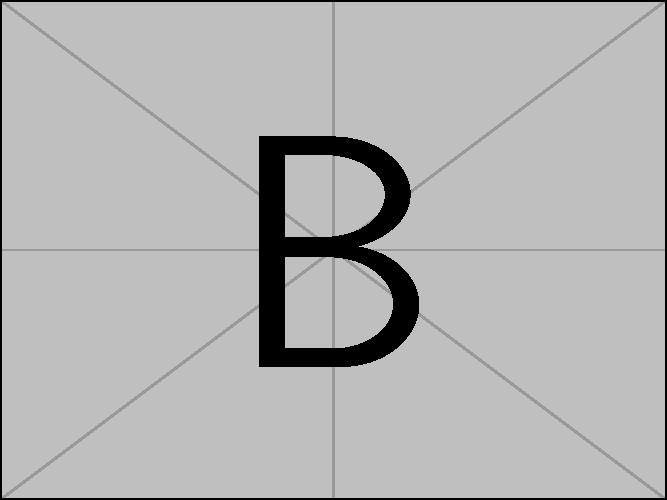
\includegraphics[width=0.45\linewidth]{example-image-b}}
\bicaption{图片标题}{English title}
\label{fig2-1}
\end{figure}

图~\ref{fig2-2}

\begin{figure}[h!t]
\centering

\includegraphics[width=0.6\linewidth]{example-image-duck}
\bicaption{图片标题}{English title}
\label{fig2-2}
\end{figure}

\section{表使用}

表~\ref{tab1}

\begin{table}[h!t]
\centering
\bicaption{表格标题}{English title}
\label{tab1}
\begin{tabular}{cc}
\toprule
Atom       & Radius(nm) \\
\midrule
Hydrogen   & 0.12       \\
Oxygen     & 0.14       \\
Nitrogen   & 0.15       \\
Carbon     & 0.17       \\
Sulfur     & 0.18       \\
Phosphorus & 0.19       \\
\bottomrule
\end{tabular}
\end{table}

表格与版心同宽 表~\ref{tab2}

\begin{table}[h!t]
\centering
\bicaption{表格标题}{English title}
\label{tab2}
\begin{tabular*}{\linewidth}{@{\extracolsep{\fill}}cccccc}
\toprule
Atom       & Radius(nm) & Atom       & Radius(nm) & Atom       & Radius(nm) \\
\midrule
Hydrogen   & 0.12       & Hydrogen   & 0.12       & Hydrogen   & 0.12       \\
Oxygen     & 0.14       & Oxygen     & 0.14       & Oxygen     & 0.14       \\
Nitrogen   & 0.15       & Nitrogen   & 0.15       & Nitrogen   & 0.15       \\
Carbon     & 0.17       & Carbon     & 0.17       & Carbon     & 0.17       \\
Sulfur     & 0.18       & Sulfur     & 0.18       & Sulfur     & 0.18       \\
Phosphorus & 0.19       & Phosphorus & 0.19       & Phosphorus & 0.19       \\
\bottomrule
\end{tabular*}
\end{table}

\section{列表使用}

有序列表

\begin{enumerate}
\item xxx
\item xxx
\item xxx
\end{enumerate}

无须列表

\begin{itemize}
\item xxx
\item xxx
\item xxx
\end{itemize}

\chapter{结论}

\zhlipsum            % 中文乱假文

% ---------------------------参考文献----------------------------------

\cleardoublepage
\addcontentsline{toc}{chapter}{参考文献}

\begin{thebibliography}{99}
\bibitem{ref1}汉娜·阿伦特著,曹明、苏婉儿译:《康德政治哲学讲稿》,上海人民出版社,2013 年 11 月版。
\bibitem{ref2}Immanuel Kant, Perpetual Peace, Unwin Brothers Ltd., 1917.
\bibitem{ref3}唐晓、王帆:《政治科学基础》,世界知识出版社,2017 年 10 月版。
\bibitem{ref4}伊曼努尔·康德著,李秋零译:《康德著作全集(第八卷)》,中国人民大学出版社,2010 年 4 月版。
\end{thebibliography} 

% ---------------------------致谢部分----------------------------------

\chapter*{致\quad 谢}
\addcontentsline{toc}{chapter}{致\quad 谢}

感谢祖国!感谢xxx

\zhlipsum[13]     % 中文乱假文

\vspace*{4.5em}

\hfill 作者

\hfill 二〇二X年于

\hfill  北京外国语大学xx学院xxx室

% ---------------------------其他信息----------------------------------

\chapter*{攻读硕士学位期间发表或录用的论文}
\addcontentsline{toc}{chapter}{攻读硕士学位期间发表或录用的论文}


\section*{一、攻读硕士期间发表的论文}

\begin{enumerate}[label={{[}\arabic*{]}},nosep]
\item xxx
\item xxx
\item xxx
\end{enumerate}

\section*{二、专利申报}

\begin{enumerate}[label={{[}\arabic*{]}},nosep]
\item xxxx
\end{enumerate}

\section*{三、参加的科研项目}

\begin{enumerate}[label={{[}\arabic*{]}},nosep]
\item xxxx
\end{enumerate}

\section*{四、科研赛事奖项}

\begin{enumerate}[label={{[}\arabic*{]}},nosep]
\item 2020年“华为杯”第xx届中国研究生数学建模竞赛 \quad \textbf{二等奖}.
\end{enumerate}

\end{document}